\documentclass{standalone}

\usepackage{amssymb}
\usepackage{amsthm}
\usepackage{amsmath}


\usepackage{tikz}
\usetikzlibrary{shapes,backgrounds,calc,patterns}
\usepackage{venndiagram}


\begin{document}
\usetikzlibrary{arrows}
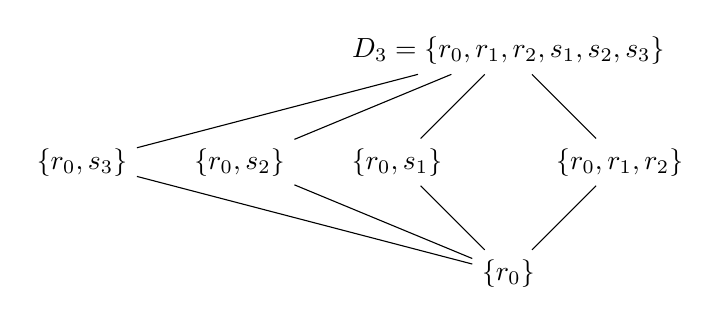
\begin{tikzpicture}[node distance=2cm]
	\node(D3) {\(D_3= \{r_0, r_1, r_2, s_1, s_2, s_3\}\)};
	\node(rot) [below right of=D3] {\(\{r_0, r_1, r_2\}\)};
	\node(s1) [below left of=D3] {\(\{r_0, s_1\}\)};
	\node(s2) [left of=s1] {\(\{r_0,s_2\}\)};
	\node(s3) [left of=s2] {\(\{r_0,s_3\}\)};
	\node(id) [below left of=rot] {\(\{r_0\}\)};
	
	\draw(D3) --(rot);
	\draw(D3) --(s1);
	\draw(D3) --(s2);
	\draw(D3) --(s3);
	\draw(s1) --(id);
	\draw(s2) --(id);
	\draw(s3) --(id);
	\draw(rot) --(id);
	
	

\end{tikzpicture}
\end{document}